%
% overview.tex
%
% Copyright (C) 2015, Achim Lösch <achim.loesch@upb.de>, Christoph Knorr <cknorr@mail.uni-paderborn.de>
% All rights reserved.
%
% This documentation may be modified and distributed under the terms
% of the BSD license. See the LICENSE file for details.
%
% encoding: UTF-8
% tab size: 4
%
% author: Achim Lösch (achim.loesch@upb.de)
% created: 7/24/14
% version: 0.5.8 - change project name to ampehre
%

\section{Component Overview}
The Ampehre project consists of several libraries and executables to provide an easy extendable modular software framework to measure various physical values such as power, energy, and temperature of integrated circuits and boards of heterogeneous high-performance computers. Figure \ref{fig:ampehre_overview} presents an overview of project components and their location in the repository's directory structure. In the following paragraph we briefly describe each component.

\begin{figure}
\begin{center}
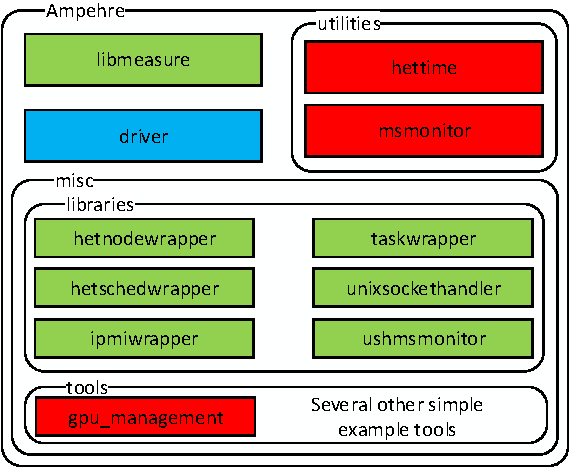
\includegraphics[width=0.8\textwidth]{ampehre_project_overview} 
\caption{Ampehre project overview showing the directory structure (rounded rectangles) and different components (green: libraries, red: executables, blue: linux kernel module).}
\label{fig:ampehre_overview}
\end{center}
\end{figure}

\begin{description}
	\item[libmeasure:] Contains the main components of the ampehre project. The measuring library consists of several modules compiled to seperate shared objects used to measure physical values such as power, energy, temperature, and utilization of resources deployed to a single heterogeneous compute node. Each of these modules implements the measuring functionality related to one of the measured resources. We describe the structure of the modules in detail in section \ref{sec:SoftwareArchitecture}. 
% 	Currently the library is made of the following resource specific modules:
% 	\begin{itemize}
% 	\item \textbf{cpu\_intel\_xeon\_sandy}: Energy, power, temperature, frequency, utilization and memory occupancy measurements.
% 	\item \textbf{fpga\_maxeler\_max3a}: Energy, power, temperature and utilization measurements.
% 	\item \textbf{gpu\_nvidia\_tesla\_kepler}: Energy, power, temperature, frequency, utilization and memory occupancy measurements.
% 	\item \textbf{mic\_intel\_knc}: Energy, power, temperature, frequency, utilization and memory occupancy measurements.
% 	\item \textbf{sys\_dell\_idrac7}: Energy, power and temperature measurements of the system board and energy and power of the complete system. 
% 	\end{itemize}
% 	
	\item[\textbf{hettime:}] Allows us to measure the energy consumption, average power dissipation, maximum device temperature, and the CPU utilization of all supported resources while executing a binary given via command line. For this the utility uses the functionality provided by the libmeasure. The results are printed to the shell or stored as a csv.
	
	\item[\textbf{msmonitor:}] Is a live monitoring tool which uses our libmeasure to retrieve current measurement values for power consumption, temperature, clock frequencies, utilization and the sum of allocated memory of the different resources. All values are shown in a Qt4-based user interface using the qwt library for plotting curves. This tool is also quite useful for debugging programms with unexpected "energy behavior".
	
	\item[driver:] Contains a dynamically loadable kernel module. Our kernel module reads CPU MSRs (Model Specific Register), memory and swap occupancy, and the CPU utilization values provided by the Linux OS. Furthermore, the kernel module allows sending IPMI (Intelligent Platform Management Interface) requests to the BMC (Baseboard Management Controller). The driver functions are available through the character device \texttt{/dev/measure}.
	
	\item[ipmiwrapper:] Provides functions to get the measured values of specific sensors via IPMI and also for DELL-specific IPMI requests. Internally, this library uses the \texttt{/dev/measure} device to send raw IPMI messages to the BMC and converts the response messages to double or integer values which are processed by the libmeasure. 
	
	\item[\textbf{gpu\_management:}] Is used to set the GPU memory and core clock frequenices and to enable or disable the Nvidia driver's persistence mode. The NVML (Nvidia Management Library) is required by the tool and is usually installed alongside Nvidia driver and CUDA packages. You can find the corresponding header file in the Nvidia GPU Deployment Kit.
	
	\item[\textbf{taskwrapper}:] Provides an interface to perform multiple energy measurements simultaneously. Since energy is the integral of power over time, we have to sample the power dissipation measured by device sensors periodically to compute a discrete approximation of the actual energy consumption. If multiple threads would perform different measurements, the same resources would be sampled concurrently, which has bad influence to the CPU load. The taskwrapper provides a simple mechanism to prevent concurrent measurements, by reading every sensor once every few milliseconds and calculating the energy consumed in the meantime individually for each registered thread. This feature can be useful, if you have one thread executing a GPU kernel while another thread is processing an FPGA kernel. This feature is less helpful, if you measure the energy consumption of multiple tasks running on the CPU simultaneously, as the energy consumption induced by one thread will invalidate the measurement result of the other task (and vice versa, of course).
	
	\item[\textbf{hetnodewrapper}:] Provides a simplified interface to the libmeasure which allows multiple measurements. Only one measurement is instantiated in the libmeasure and the values of this measurement are sampled by the hetnodewrapper at the beginning and end of every measurement. The subtractions of the particular final and first measurements are the actual result used for returned measurements. The library retrieves runtime, energy, and utilization measurements for CPU, GPU, FPGA, and the mainboard respectively power supply.
	
	\item[\textbf{hetschedwrapper}:] Uses the taskwrapper for measurements providing a more abstract interface. The wrapper is used by an external project not embedded in this repository.
	
	\item[\textbf{unixsockethandler:}] Implements a communication layer for client-server IPC, based on Unix sockets with the advantage of a simple interface hiding the system calls.
	
	\item[\textbf{ushmsmonitor:}] Is a library enhancing the general-purpose Unix socket-based IPC implementation of the unixsockethandler library. Our msmonitor monitoring utility uses the ushmsmonitor library as a server listening to a Unix socket. A client such as hettime must implement the counterpart. The clients can transmit start and stop signals to the server. Accordingly, servers are able to perform any activity after receiving these signals. For instance, out msmonitor tool shows start and stop markers on the qwt plots as well as the client's PID sending the corresponding signals.
\end{description}

Additionally, the \texttt{/misc/tools} directory contains several simple example programs which use the mentioned libraries. Each executable allows us to test a specific functionality of our project. \textbf{The \texttt{example\_ms} tool shows all function calls which are necessary to perform measurements with our measuring library.}
